Die Implementation einer geregelten Geradeausfahrt eines Roboters braucht ein paar Schritte. Zuerst muss ein funktionierdes Modell des Roboters gefunden werden. Danach muss irgendeine Querabweichung ber"ucksichtigt werden. Am Ende kann ein Regler f"ur das System gefunden werden. 

\subsection{Linearisierung in $X_2$-Richtung}

Die folgende Modellgleichung eines einachsigen Roboters wird gegeben:
\begin{equation} \label{eq:model}
    \overrightarrow{f}(\overrightarrow{x}, \overrightarrow{u}) =
    \begin{bmatrix*}
        \dot{x}_1 \\
        \dot{x}_2 \\
        \dot{x}_3
    \end{bmatrix*}
    =
    \begin{bmatrix*}
        \sin(x_3) & 0 \\
        \cos(x_3) & 0 \\
        0 & 1
    \end{bmatrix*}
    \begin{bmatrix*}
        v \\
        \omega
    \end{bmatrix*}
\end{equation}. \\

Wegen des nichtlinearen Forms der Modellgleichung ist es schwierig das Systemverhalten des Modells zu beobachten. Deshalb wird sie in einem Arbeitspunkt linearisiert und dann wird dieses Modells betrachtet. Im Folge ist die Herleitung des linearisierten Modells:
\begin{equation}
    \overrightarrow{\widetilde{f}}(\overrightarrow{\widetilde{x}}, \overrightarrow{\widetilde{u}}) =
    \begin{bmatrix*}
        \dot{x}_1 \\
        \dot{x}_2 \\
        \dot{x}_3
    \end{bmatrix*}
    =
    \begin{bmatrix*}
        0 & 0 & \cos(x_{30})v_0 \\
        0 & 0 & -\sin(x_{30})v_0 \\
        0 & 0 & 0
    \end{bmatrix*}
    \begin{bmatrix*}
        \widetilde{x_1} \\
        \widetilde{x_2} \\
        \widetilde{x_3} 
    \end{bmatrix*}
    +
    \begin{bmatrix*}
        \sin(x_{30}) & 0 \\
        \cos(x_{30}) & 0 \\
        0 & 1
    \end{bmatrix*}
    \begin{bmatrix*}
        \widetilde{v} \\
        \widetilde{\omega}
    \end{bmatrix*}
\end{equation}.
Mit
\begin{equation*}
    \overrightarrow{\widetilde{x}} =
    \begin{bmatrix*} 
        x_1 - x_{10} \\
        x_2 - x_{20} \\
        x_3 - x_{30} 
    \end{bmatrix*}
    =
    \begin{bmatrix*} 
        \widetilde{x_1} \\
        \widetilde{x_2} \\
        \widetilde{x_3} 
    \end{bmatrix*},
    \overrightarrow{\widetilde{u}} =
    \begin{bmatrix*}
        v - v_0\\
        \omega - \omega_0
    \end{bmatrix*}
    =
    \begin{bmatrix*}
        \widetilde{v} \\
        \widetilde{\omega}
    \end{bmatrix*},
\end{equation*}
\(x_{10}\) und \(x_{20}\) sind die Komponenten des Vektors, wo der Roboter startet. Die k"onnen dann auf 0 gesetzt werden. \(x_{30}\) ist der Anfangswinkel des Roboters, welche hier \si{0\degree} ist. Die obere Gleichung l"asst sich dann in der folgenden Gleichung vereinfachen:
\begin{equation}
    \widetilde{f}(\overrightarrow{\widetilde{x}}, \overrightarrow{\widetilde{u}}) =
    \begin{bmatrix*}
        \dot{x}_1 \\
        \dot{x}_2 \\
        \dot{x}_3
    \end{bmatrix*}
    = 
    \begin{bmatrix*}
        v_0\widetilde{x_3} \\
        \widetilde{v} \\
        \widetilde{\omega}
    \end{bmatrix*}
\end{equation}

\subsection{Querabweichung}

In der reellen Welt kann der Roboter nicht perfekt gerade fahren und hat einen kleinen Winkel von der \(X_2\)-Richtung. Deshalb muss die Querabweichung der Fahrt ber"ucksichtigt werden. Die Querabweichung \(\overrightarrow{e}\) ist als der Vektor zwischen dem geplanten Zielpunkt \(\overrightarrow{r}\) und der jetztigen Endposition \(\overrightarrow{x}\) des Roboters definiert, wie in der folgenden Gleichung gezeigt wird:
\begin{equation*}
    \overrightarrow{e} = \overrightarrow{x} - \overrightarrow{r}.
\end{equation*} \\

Der Zielpunkt \(\overrightarrow{r}\) ist bei der Geradeausfahrt nur die \(X_2\)-Komponent des Positionsvectors.  Die Gleichung im Vector-Form wird in der folgenden Gleichung gezeigt:
\begin{equation*}
    \begin{bmatrix}
        x_1 \\
        x_2 \\
        0
    \end{bmatrix}
    -
    \begin{bmatrix}
        0 \\
        x_2 \\
        0
    \end{bmatrix}
    =
    \begin{bmatrix}
        x_1 \\
        0 \\
        0
    \end{bmatrix}
\end{equation*}.

Die obere Gleichung l"asst sich mit der folgenden eindimensionalen Gleichung vereinfachen:

\begin{equation}
    e(t) = x_1(t).
\end{equation}

Bei der ersten Ableitung der oberen Gleichung nach der Zeit wird der Zussamenhang zwischen der Querabweichung und dem Modell gezeigt. Der Zussamenhang ist in den folgenden Differentialgleichungen gezeigt:

\begin{align}
    \dot{e} &= \dot{x}_1 = v_0\widetilde{x}_3(t) \nonumber \\
    \ddot{e} &= v_0\dot{\widetilde{x}}_3(t) = v_0\omega(t) \label{diff_eq}
\end{align}

\subsection{Wurzelortskurven}    

Um das Systemverhalten mit verschiedenen Reglertypen zu untersuchen, muss der Differentialgleichung \ref{diff_eq} zu einer "Ubertragungsfunktion transformiert werden. Mit der Laplacetransformation wird
\begin{equation}
    P(s) = \frac{E(s)}{\Omega(s)} = \frac{v_0}{s^2}
\end{equation}
erhaltet.

Mit einem Pythonskript wird die Strecke nun untersucht. Die 

\begin{figure}
    \centering
    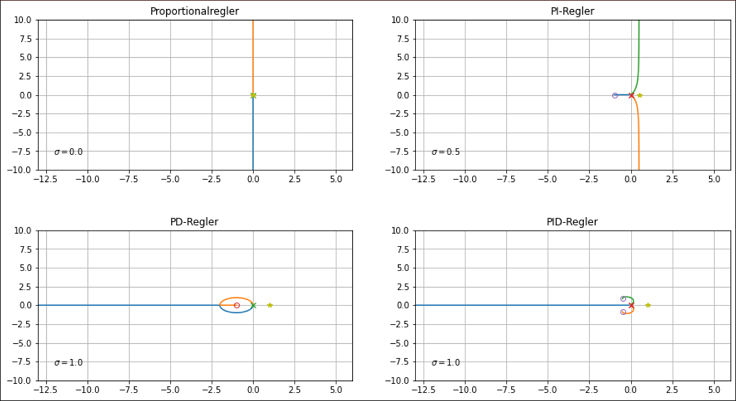
\includegraphics{root_locus}
    \caption{Wurzelortskurven}
    \label{fig:root_locus}
\end{figure}

\subsection{Implementation}

Zur Zeit des Abschliessens dieser Seminararbeit k"onnte eine funktionierende Implementation der geregelten Geradeausfahrt nicht gefunden werden. Mehr Information steht im Kapitel 6. \\




